\begin{figure}[t]
    \centering
    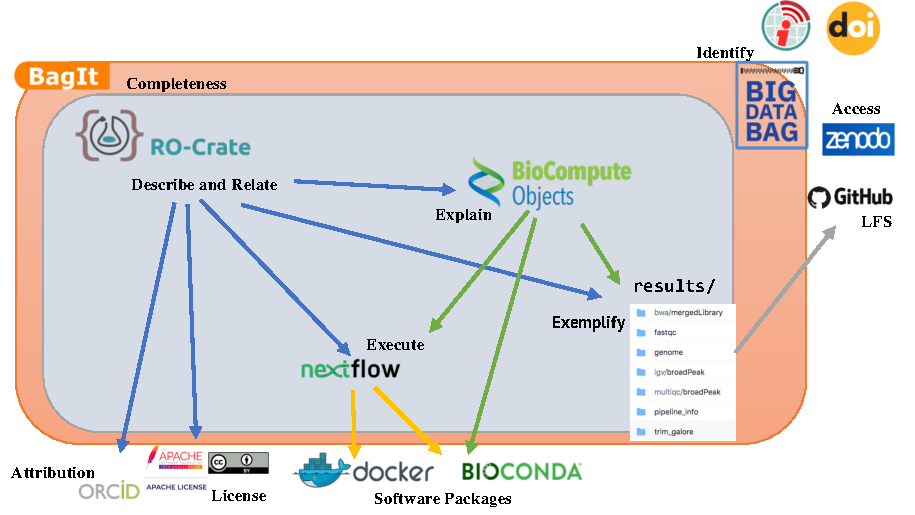
\includegraphics{content/images/ro-crate-bco-sep-of-concerns.pdf}
    \caption{\textbf{Separation of Concerns in BCO RO-Crate}. BioCompute Object (IEEE2791) is a JSON file that structurally explains the purpose and implementation of a computational workflow, for instance implemented in Common Workflow Language (CWL), that installs the workflow’s software dependencies as Docker containers or BioConda packages. An example execution of the workflow shows the different kinds of result outputs, which may be external, using GitHub LFS to support larger data. RO-Crate gathers all these local and external resources, relating them and giving individual descriptions, for instance permanent DOI identifiers for reused datasets accessed from Zenodo, but also adding external identifiers to attribute authors using ORCID or to identify which licences apply to individual resources. The RO-Crate and its local files are captured in a BagIt whose checksum ensures completeness, combined with Big Data Bag \cite{doi:10.1109/BigData.2016.7840618} features to “complete” the bag with large external files such as the workflow outputs.}
    \label{fig:sep_concerns}
\end{figure}